\documentclass[border=3mm]{standalone}
\usepackage{tikz}
\usetikzlibrary{circuits.logic.US}

\begin{document}
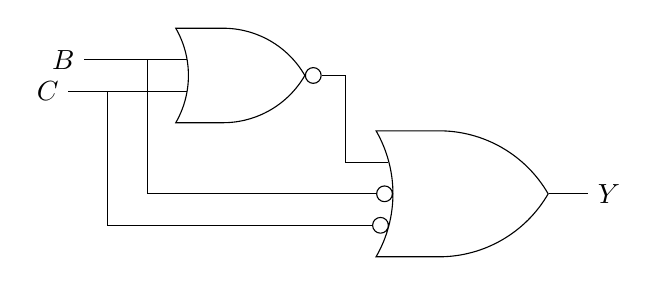
\begin{tikzpicture}[circuit logic US,
                    tiny circuit symbols,
                    every circuit symbol/.style={fill=white,draw,logic gate input sep=4mm, logic gate inverted radius=1mm}
]

\node [nor gate, inputs = nn] at (0,0) (nor1) {};
%\node [and gate, inputs = in] at ($(nor1.south) + (0,2.0cm)$) (and2) {};
\node [or gate, inputs = nii, anchor=input 1] at ($(nor1.south)+(2.0cm,-0.5cm)$) (or1) {};
%
\draw (nor1.input 1) -- ++(left:13mm) node[left] (B) {$B$};
\draw (nor1.input 2) -- ++(left:15mm) node[left] (C) {$C$};
%\node (C) at (A|-or1.input 2) {$C$};
%\draw (or1.input 1) -- (C);
\draw (nor1.output) -- ++(right:3mm) |- (or1.input 1);
\draw (or1.output) -- ++(right:5mm) node[right] (Y) {$Y$};
%
\draw (nor1.input 1) -- ++(left:5mm) |- (or1.input 2);
\draw (nor1.input 2) -- ++(left:10mm) |- (or1.input 3);
%\draw (and2.output) -- ++(right:7mm) |- (or1.input 1);
\end{tikzpicture}
\end{document}
